\section{Tracer particles}

Tracer particles are to track the Lagrangian evolution of a model fluid using discrete particles. In hydrodynamical simulations based on an Eulerian grid (including CASTRO), thermodynamic variables at a given time are derived by solving the equations of motion of a fluid between cells. Therefore, in this scheme, the physical quantities that we can access to are not discretized quantities at any given position, but rather average values over each cell. However, employing discrete particles, passively advected with the fluid flow, allows us to obtain local instantaneous thermodynamic variables, such as the temperature and the density, at well-defined positions, independent of the spatial resolution, i.e., the spatial cell size. This means that we can follow the evolution of the fluid at any given position and time. 

\noindent \noindent CASTRO provides a tracer particle scheme with useful options. In this scheme, particles are advanced using the midpoint method either with the cell-centered velocities or the face-centered velocities (Marker-And-Cell method)\footnote{One can simplify interpolation with the cell-centered velocity. However, this can lead to decoupling of the pressure and the velocity components, possibly resulting in instability. This can be avoided with the face-centered velocity}. The number and the initial positions of particles are flexibly determined according to the purpose of a given model. 


\section{Initializing the Particles}

One must include the tracer particles in the {\tt GNUmakefile} by setting

\vspace{0.1in}
\noindent{\tt USE\_PARTICLES = TRUE}.
\vspace{0.1in}

\noindent And the particles can be initialized via

\vspace{0.1in}
\noindent {\tt {\bf castro.do\_tracer\_particles }}     = 1
\vspace{0.1in}

\noindent in the {\tt {\bf inputs}} file.

If one wants to investigate the evolution of fluid motions starting from specific positions (or a certain range of area or volume), one should manually specify the positions of particles by providing an input file containing the total number and the initial positions of the particles.  
The input file should be in the same directory where your {\tt inputs} file is located. The name of the input file is  determined via :

\vspace{0.1in}
\noindent {\tt {\bf particles.particle\_init\_file =}}{\em particle\_file}
\vspace{0.1in}

\noindent Here {\em particle\_file} is the user-specified name of the file. The first line in this file is
assumed to contain the number of particles.  Each line after that contains the positions in a coordinate system adopted for your model. For 3-D cartesian coordinates, \\

$x ~y ~z$ \\

For example, an input file for a model fluid with 6 particles in 2-D Cartesian coordinates may look like,\\

\begin{lstlisting}
6
3.28125e+08 9.9198e+08 
5.46875e+08 9.9198e+08 
7.65625e+08 9.9198e+08 
9.84375e+08 9.9198e+08 
1.20312e+09 9.9198e+08 
1.42188e+09 9.9198e+08 
\end{lstlisting}

According to this input file, the 6 particles will be positioned at the same height (same $y$ coordinate in the second column), equally spaced in $x$ direction (the first column except for the particle number on the first line) from $3.28\times10^{8} {\rm ~cm}$ to $1.42\times 10^{9} {\rm ~cm}$.





\section{Output file}
\label{particles:output_file}
\noindent The output files are stored in a directory whose name is determined by a variable {\tt particles.timestamp\_dir}. For example, if the variable is set as follows,

\vspace{0.1in}
{\tt  {\bf particles.timestamp\_dir=}} {\em particle\_dir},
\vspace{0.1in}

\noindent A directory {\em particle\_dir} is automatically made with the directories for the main CASTRO output file ({\tt plt****}) once a simulation starts and the particle output files are stored inside that directory.

\vspace{0.05in}
\noindent The name of the output file consists of {\tt Timestamp\_} along with a number at the end. The number increases (typically from 00) as more processors are involved in following the trajectories of particles. In parallel computing, a computational domain is divided according to the number of processors requested. Then each processor only follows the particles on the domain assigned to that processor and records their positions and velocities at any given time in a different output file. Since it is possible for particles to move from one domain to another during the evolution, its history can be stored in different files. More output files (with larger numbers at the end of the file name) can be produced as more processors track the particles.  

\vspace{0.05in}
\noindent By default, the output file contains the positions and velocities of all particles at a given time, meaning [$3+ 2\times$dimensionality] columns. For example, for particles in a 3-D domain, the columns in the output file are, 

\vspace{0.1in}
${\rm index1}~~{\rm index2}~~x~~ y~~ z~~ t~~ v_{\rm x} ~~v_{\rm y}~~ v_{\rm z}~~ [\rho ~~ T]$
\vspace{0.1in}

\noindent The first two integers correspond to the particle index and the processor number. 
One should use the two numbers in order to identify a particle and extract its history (i.e., the trajectory in Figure \ref{fig:particletrajectory}). 

\begin{figure}[h]
	\centering
	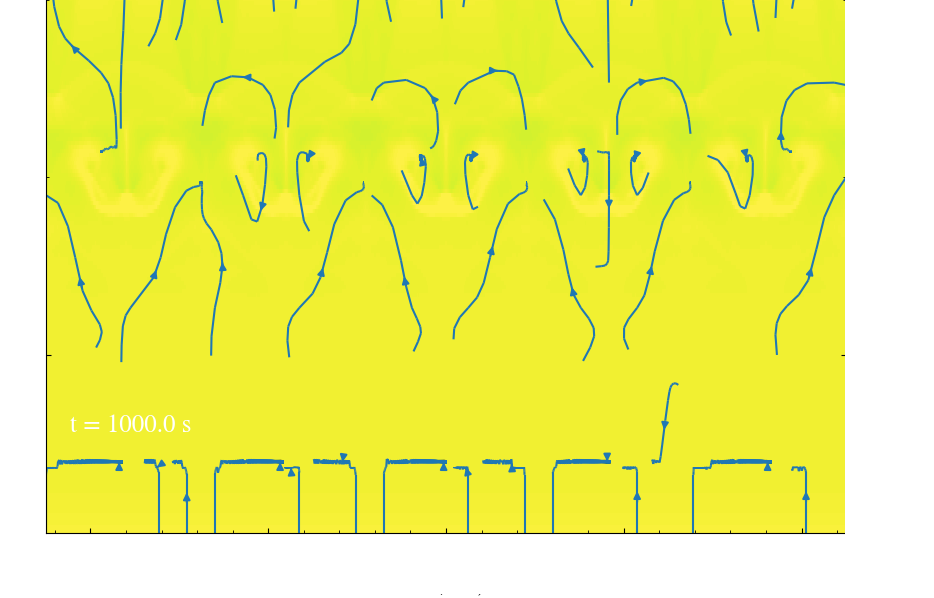
\includegraphics[width=2.5in]{fluid_motion}
	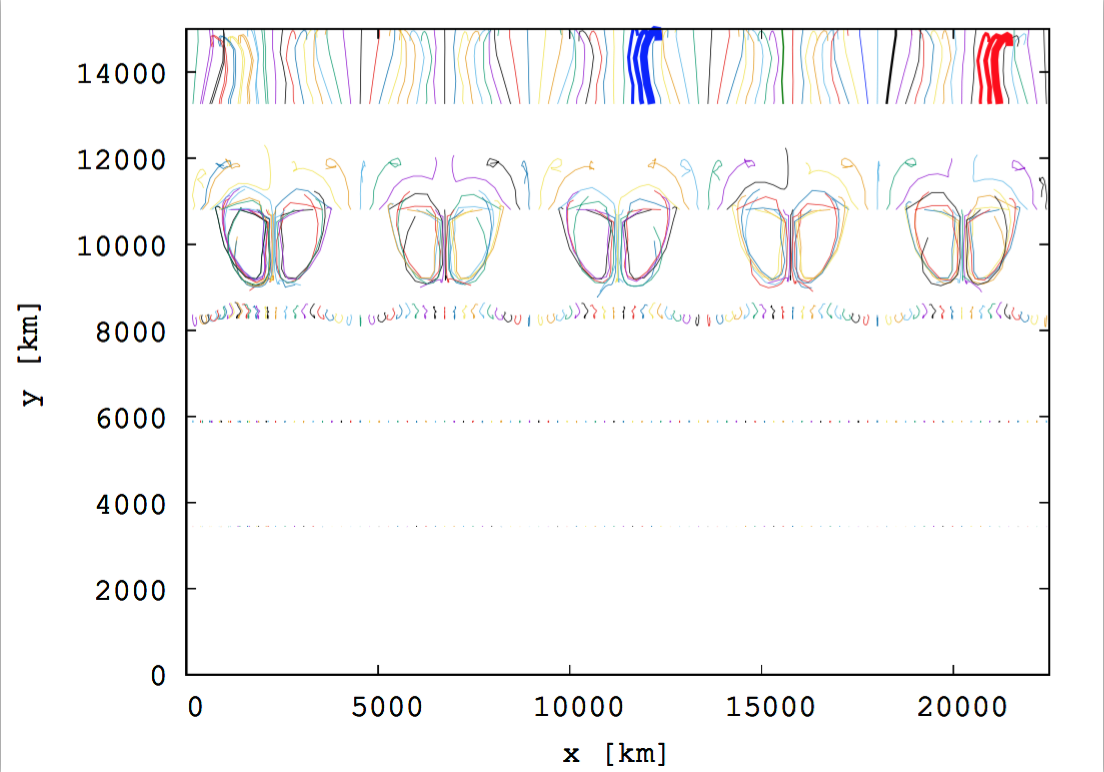
\includegraphics[width=2.39in]{tracer_trajectory}
	\caption{A model atmosphere (\textit{left} panel) and the trajectories of 500 particles (\textit{right} panel) following the fluid motion on the atmosphere. The particles are initially positioned at five different heights, $y=13000\mathrm{~km},~11000\mathrm{~km},~ 8000\mathrm{~km},~ 6000\mathrm{~km}, ~38000\mathrm{~km}$ (100 particles at each height). In the \textit{left} panel, the arrows roughly show the fluid motion. In the \textit{right} panel, the solid lines represent the trajectories of the particles. }
	\label{fig:particletrajectory}
\end{figure}



\noindent One can also add the last two columns $[\rho ~~ T]$, i.e., the local density and local temperature of fluid at the position of each particle by setting the following,

\vspace{0.1in}
\noindent {\tt {\bf particles.timestamp\_temperature }}= 1,\\
\noindent {\tt  {\bf  particles.timestamp\_density}}     = 1.
\vspace{0.1in}

\noindent For example, let's consider 10 particles on a domain.  If 4 out 10 particles are initially on a processor and the rest are on another processor, this means two processors are tracking the particles and two output files are produced. In the output file written by the processor with 4 particles, one can find that four lines are stored at the same time and each line corresponds to each particle info. while in the other output file for the other 6 particles, 6 lines are stored at the same time. 



\vspace{0.05in}

\noindent If {\tt {\bf particles.write\_in\_plotfile=1}}, the particle data are stored in a binary file along with the main CASTRO output plotfile in directories {\tt plt*****/Tracer/}. 
\vspace{0.05in}




\subsection{Run-time Screen Output}

The verbosity written to the screen at run-time is constrolled by setting:

\noindent {\bf particles.v } = 0 or 1 (default: 0)\\
